\documentclass[25pt, a0paper, portrait]{tikzposter}
\usepackage{blindtext}
\usepackage{comment}
\graphicspath{{figures/}}

\title{Tikz Poster Example}
\author{ShareLaTeX Team}
\date{\today}
\institute{ShareTeX Institute}

\usetheme{Board}
\begin{document}

\maketitle

\block{preambles}
{
    Available font sizes: 12pt, 14pt, 17pt, 20pt, 24pt.	\\
    Possible paper sizes: a0paper, a1paper and a2paper.	\\
    Orientation: portrait, landscape. \\
}

\begin{columns}
    \column{0.4}
    \block{Column1}
    {
	In \textbf{tikzposter} the text is organized in blocks, each
	block is created by the command \textbackslash{}block\{\}\{\}.  \\
	To insert figures in the \textbf{tikzposter}, use \textbf{tikzfigure}
	environment.
    }

    \column{0.6}
    \block{Column2}
    {
	\textbackslash{}note[]\{\} is used to add additional notes that are rendered
	overlapping the text block. \\

	\vspace{3cm}
    }
    \note[
	targetoffsetx=-9cm,
	targetoffsety=-1.5cm,
	width=0.5\linewidth,
    ]
    {email \texttt{abc@example.com}}
\end{columns}

\begin{columns}
    \column{0.25}
    \block{Default}
    {
	\begin{tikzfigure}
	    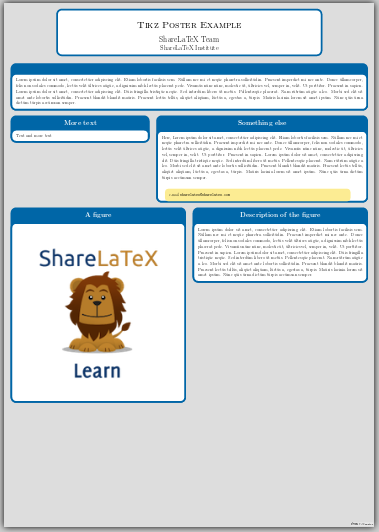
\includegraphics[width=\linewidth]{Tikzposter_theme/Default}
	\end{tikzfigure}
    }
    \column{0.25}
    \block{Rays}
    {
	\begin{tikzfigure}
	    
\includegraphics[width=\linewidth]{Tikzposter_theme/Rays}
	\end{tikzfigure}
    }
    \column{0.25}
    \block{Basic}
    {
	\begin{tikzfigure}
	    
\includegraphics[width=\linewidth]{Tikzposter_theme/Basic}
	\end{tikzfigure}
    }
    \column{0.25}
    \block{Simple}
    {
	\begin{tikzfigure}
	    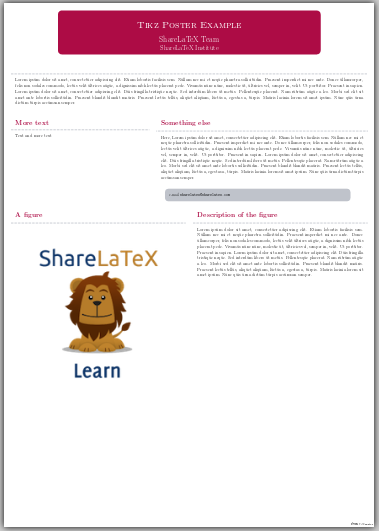
\includegraphics[width=\linewidth]{Tikzposter_theme/Simple}
	\end{tikzfigure}
    }
\end{columns}

\begin{columns}
    \column{0.2}
    \block{Envelope}
    {
	\begin{tikzfigure}
	    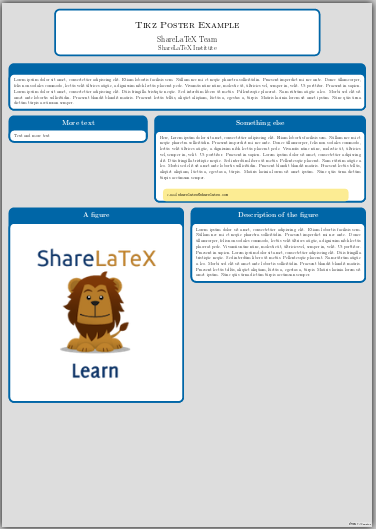
\includegraphics[width=\linewidth]{Tikzposter_theme/Envelope}
	\end{tikzfigure}
    }
    \column{0.2}
    \block{Wave}
    {
	\begin{tikzfigure}
	    
\includegraphics[width=\linewidth]{Tikzposter_theme/Wave}
	\end{tikzfigure}
    }
    \column{0.2}
    \block{Board}
    {
	\begin{tikzfigure}
	    
\includegraphics[width=\linewidth]{Tikzposter_theme/Board}
	\end{tikzfigure}
    }
    \column{0.2}
    \block{Autum}
    {
	\begin{tikzfigure}
	    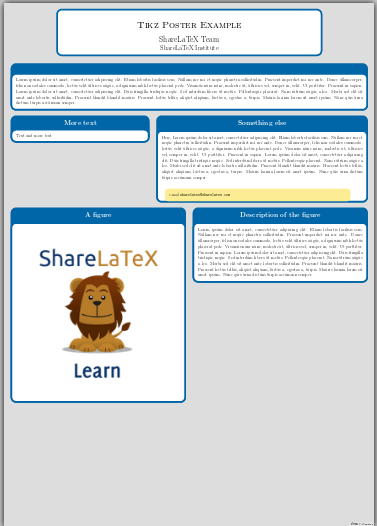
\includegraphics[width=\linewidth]{Tikzposter_theme/Autum}
	\end{tikzfigure}
    }
    \column{0.2}
    \block{Desert}
    {
	\begin{tikzfigure}
	    
\includegraphics[width=\linewidth]{Tikzposter_theme/Desert}
	\end{tikzfigure}
    }
\end{columns}
\end{document}
